\chapter{Evolutionary Algorithms} % top level followed by section, subsection

%: ----------------------- paths to graphics ------------------------

% change according to folder and file names
\ifpdf
    \graphicspath{{2/figures/PNG/}{2/figures/PDF/}{2/figures/}}
\else
    \graphicspath{{2/figures/EPS/}{2/figures/}}
\fi

%: ----------------------- contents from here ------------------------

\begin{flushright}
Life results from the non-random survival 
\linebreak
of randomly varying replicators.
\linebreak
Richard Dawkins 
\end{flushright}
\section{Evolutionary Algorithms}
The ever increasing computational power and its availability with relatively low cost has transformed stochastic optimization methods into valid industrial design tools. A number of stochastic optimization methods based on the ideas presented   
in Darwin's theory of evolution on the origin of species \cite{Darwin} have been proposed over the years \cite{Back1996}. During the 60s evolutionary programming was proposed by Fogel \cite{Fogel} and evolutionary strategies by Rechenberg \cite{Rechenberg} as engineering problem solving techniques. During the same period genetic algorithms were proposed by Holland \cite{holland_1975} as evolution emulating tools. Genetic programming was proposed significantly later by Crammer \cite{cramer85} and improved by Koza \cite{Koz94} aiming in automated design of computer programs given as input the problem that has to be resolved. The aforementioned algorithms in-spite of their differences can be placed in a common group named Evolutionary Algorithms (EA) \cite{Back1996}. 


The main EA characteristics are the population based evolution and the fact that the inheritance of genotype is based on probabilistic criteria and the decisions made based upon a fitness function quantifying the ability of each individual to survive in a given environment, where environment is a function of the optimization objectives. Evolution, from each generation to the next, fig~\ref{EA}, is achieved with the use of evolution operators, inspired from Darwin's theory of evolution, namely recombination, elitism, mutation, etc. 

The need to evaluate all the individuals in the population, in order to assign individual fitness values according to the environment, is the main drawback of EAs when dealing with industrial engineering optimization problems. This is due to the high computational cost of each individual fitness-assignment, making the overall computational cost for each optimization quite high resulting in unacceptable wall time for each problem. To tackle this a number of techniques have been proposed in literature. The massive parallel processing is relatively easy to implement due to the population nature of the algorithm, on top of that asynchronous EAs \cite{LTT_2_040} where developed to achieve grater usage of the available computational resources.  An efficient way to reduce the computational cost is the employment of metamodels \cite{EBNK,KCGVKI04}. Metamodels are either interpolation/approximation tools that can approximate/predict the individual's fitness value \cite{LTT_4_05,LTT_2_029}, or pattern recognition tools that can recognise if the individual genotype (pattern) is promising or not \cite{KCGVKI00a,KCGVKI00b}. Furthermore Hierarchical EAs \cite{LTT_2_044} were devised to accommodate the availability of; a) a number of evaluation tools with different fidelity and ofcource different cost, b) a number of different parametrization levels and c) a number of different optimization methods.      

\figuremacroW{EA}{EA schematic representation }{This figure shows a schematic representation of the evolutionary algorithm. Each population is derived by the previous one via evolution operators i.e. parent selection, crossover and mutation }{0.8}

\subsection{Optimization problem}
Optimization problems in general can be formulated as:
\begin{align} 
   &min ~ F(x)=(f_1(x),f_1(x),...,f_M(x))\in \Re^{M} \nonumber \\
   &\mbox{subject to} ~ c_k(x)\leq d_k ~ k =1,K
\label{OptimIN}
\end{align}
where $x\in X \!\leq\! \Re^{N}$ is the design vector and $X$ the design space. If equality constraints are enforced $ c^*(x)=d^* $, they can be transformed into inequality constraints $ c(x)=\Vert c^*(x)-d^*\Vert \leq d $ where $ d \in \Re $ a very small number.  Problem \ref{OptimIN} becomes a multi-objective optimization problem if $M \!> \!1$, in such case the notion of Pareto dominality \cite{Zitzler2000} is used to define each individuals fitness and the EA will deliver Pareto fronts of non-dominated individuals as result. 

\subsubsection{Multi Objective optimization problem}
Problem \ref{OptimIN} is, in its general form a multi-objective problem. If a solution $\vec{x}$ that simultaneously minimizes all objectives exist then this is the overall solution of \ref{OptimIN}. In case of contradictive objectives though Pareto front dominality is in use.

\paragraph{Pareto Dominality} Solution $\overrightarrow{x_1}$ dominates solution $\vec{x_2}$ ($\vec{x_1}\prec\vec{x_2}$) if and only if it has better (smaller for minimization problems) or equal value for all objectives and at least one with better value in respect to $\vec{F}(\vec{x_2})$.

\begin{eqnarray}
    \vec{x_1}\prec\vec{x_2} \Leftrightarrow (\forall _i :  f_i(x_1) \leq f_i(x_2))\wedge (\exists _i : f_i(x_1) < f_i(x_2))
   \label{pareto_eq} 
\end{eqnarray}

\paragraph{Pareto optimal solution} Solution  $\vec{x_1}$ is a Pareto optimal solution if and only if it is not dominated by any other solution.% Hence the Pareto optimal front is also known as the front of non-dominated solutions.  


\begin{eqnarray}
    \nexists\vec{x}:\vec{x}\prec\vec{x_1}
\end{eqnarray}
 
\figuremacroW{Pareto2}{}{Schematic representation of Pareto dominality. $\vec{x_1}$ is a Pareto optimal solution since it is not dominated by any other solution furthermore $\vec{x_1}$ itself dominates all individuals located in the grey box.}{0.7}

Assuming that the individuals shown in fig. \ref{Pareto2} is the population of an EA generation, with black points the current front of non-dominated individuals is noted and with white points all the dominated individuals. Furthermore the area dominated by $\vec{x_1}$ is shown in grey, the individuals located in the grey area are dominated at least by $\vec{x_1}$. 

\paragraph{Fitness assignment for multi-objective problems.}
Even though for single-objective optimization fitness assignment is equivalent with the one objective ($\Phi(\vec{x})=F(\vec{x})$) in multi-objective problems things are different. In multi-objective problems a procedure is needed to reduce the $M$-dimentional vector of objectives $\vec{F}(\vec{x})$ into a scalar metric $\Phi(\vec{x})$ that will represent the individual's fitness. 

\begin{eqnarray}
    \Phi(\vec{x})=\Phi(\vec{F}(\vec{x})) :\Re ^M \rightarrow \Re ^1 
\end{eqnarray}

There is a lot of different algorithms proposed in literature that offer this ability. A complete review of literature on the subject can be found in \cite{CoCo99,coe02,Miett99}. Furthermore the Strength Pareto Evolutionary Algorithm II (SPEA II), that is used in this thesis, is presented here \cite{Zitz01,Zitz02}.

\paragraph{SPEA II}
is an improvement over SPEA \cite{ZiTh98}. The improvements consist on the additional information about the number of dominated, by the currently evaluated individual, individuals as well as the one that dominate it. The use of density information additionally helps the better distribution of the individuals on the Pareto front (traditional SPEA had a bias of favouring the individuals located in the middle of the Pareto). 

\subparagraph{} In SPEAII algorithm, strength value of individual $i$ ($S_i$) is defined as the sum of the population members that are dominated or equal to $i$, with respect to the objective functions, divided by the total number of the individuals in the population.  


\subparagraph{SPEA II algorithm}

\begin{itemize}
\item[]{\bf step 1:}  (Strength calculation), the strength of every member of the population $P$ is computed. 
\begin{eqnarray}
	\nonumber
	\forall i \in P = P_{\lambda}^g \cup P_{\mu}^g \cup P_{e}^g  
\end{eqnarray}
\begin{eqnarray}
	S_i = \frac{\sum(j : j \in P \wedge i \prec j)} {\sum P} 
\end{eqnarray}

\item[]{\bf step 2:}  (Density calculation), the density metric is calculated for each member of the population, defined as the distance between it and its closest neighbour.

\begin{eqnarray}
	D_i = \frac{1} {d_i+2} 
\end{eqnarray}
where
\begin{eqnarray}
	\nonumber
	d_i= min (\parallel \vec{F_i} - \vec{F_k} \parallel), ~ k \in P  
\end{eqnarray}


\item[]{\bf step 3:}  (fitness calculation), the fitness value for all the members of the population is calculated as the sum of raw fitness $R_i$ and the density metric.

\begin{eqnarray}
	\Phi_i = R_i+D_i
\label{SPEAIIeq}
\end{eqnarray}
here $R_i$ is the sum of the individual strengths of the population members that dominate it,
  
\begin{eqnarray}
	\nonumber
	R_i=\sum _{j \in P \wedge i \prec j}(S_j)  
\end{eqnarray}  
\end{itemize}

\paragraph{Performance metric for multi-objective optimization problems}
A quality measure of Pareto fronts is needed for the comparison of the performance of different optimization multi-objective optimization techniques. In this thesis the Hypervolume indicator is chosen for that purpose \cite{zbt2007a}. Hypervolume indicator assumes that the quality of a Pareto front can be quantified in a scalar value, the hypervolume of the dominated by the Pareto front portion of the objective space restricted by reference point $\vec{b}$ as defined in eq.\ref{hyperVeq}. 

The hypervolume indicator of a set $A$  and reference point $(b_1,...,b_M)$ is defined as:
\begin{eqnarray}
	I(A,b)=\int _{(0,...,0}^{(b_1,...,b_M)}a_A(x)dx 
\label{hyperVeq}
\end{eqnarray}  
where,

\begin{eqnarray}
	\nonumber
	a_A(x) = \left\{ \begin{array}{ll}
    1 & \mbox{if $(A\prec{x})$}\\
    0 & \mbox{else}\end{array} \right.
    ,~x\in A
\end{eqnarray}    


\begin{figure}[h!]
\begin{minipage}[b]{0.5\linewidth}
 \centering
 \resizebox*{6.5cm}{!}{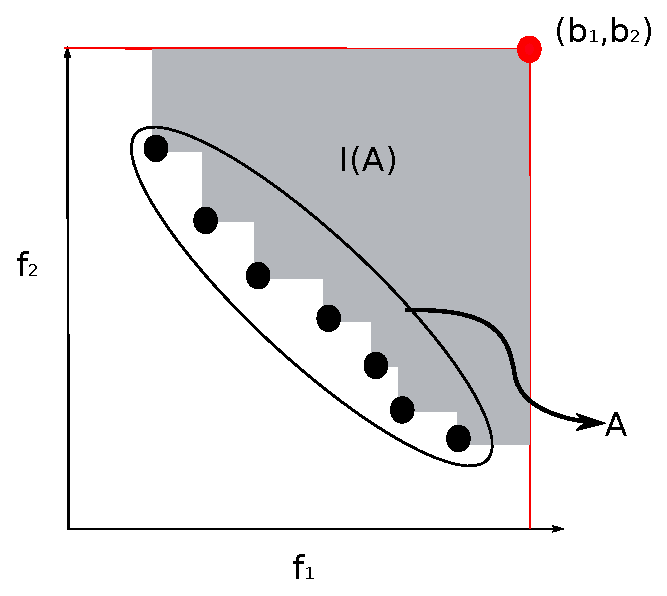
\includegraphics{hyperVol.eps}}
\end{minipage}
\begin{minipage}[b]{0.5\linewidth}
 \centering
 \resizebox*{9.0cm}{!}{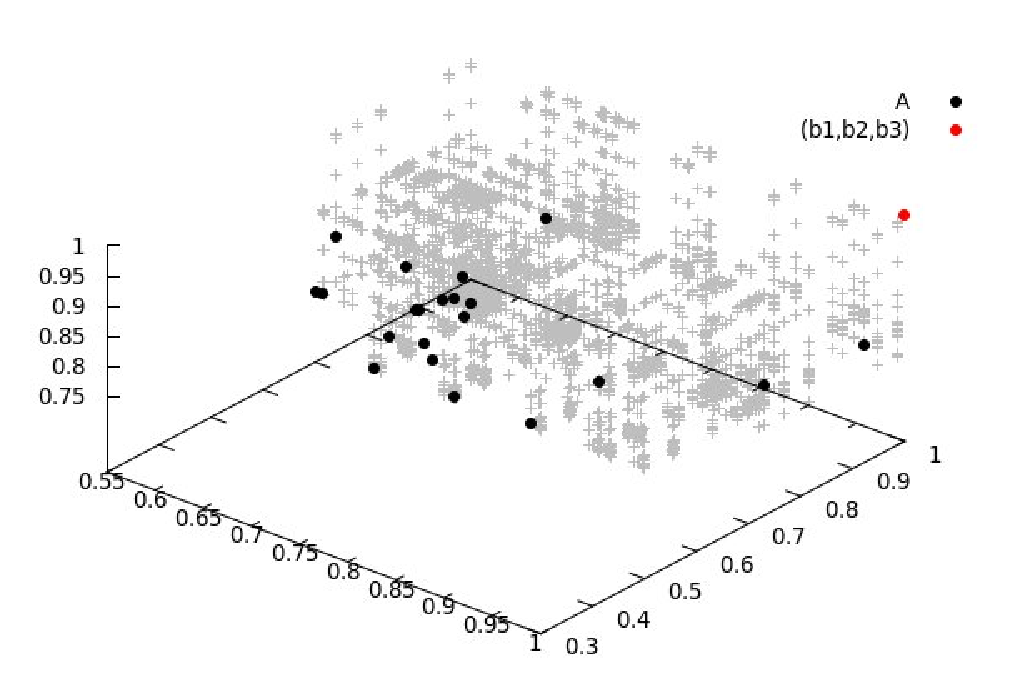
\includegraphics{pareto3d.eps}}
\end{minipage}
\caption{Two dimensional (left) and three dimensional (right) examples of hypervolue indicatror for set $A$. Reference point is $(b_1,...,b_M)$.}
\label{hyperV}
\end{figure}

Given that the same $\vec{b}$ is used two Pareto-fronts can be compared using there Hypervolume indicators. Pareto front ($i$) is better from Pareto front ($j$) if the Hypervolume indicators of ($i$) is grater that the Hypervolume indicators of ($j$), 

\begin{eqnarray}
   i\prec j \leftrightarrow I(A_i,b) > I(A_j,b)
\end{eqnarray}    


\subsubsection{Constrained optimization problem}
EAs are not inherently built to handle constrained optimization problems. In engineering cases, though, it is usual for a number of constraints to govern the optimization problem in hand. The most common way to deal with constraints in an EA environment is a) the use of penalty functions \cite{Deb00,morales98} assigning evolutionary advantages to the individuals that satisfy the constraints \cite{powell93}, b) the conversion of constraints into objectives \cite{surry95,surry97} and c) the use of correction operators \cite{mich94}. Detailed literature survey on this subject can me found in \cite{mich96,coello02}.

In this thesis an improved version of the penalty functions technique is in use. In the traditional penalty functions technique EA takes into account the constraints by adding penalty terms (proportional to the magnitude of the constraint violation) on the objectives. For each constraint in addition to the hard limit ($d$, the constraint value as described by the optimization problem) a "relaxed limit" $d_k^*$ is also introduced. Once an individual violates the relaxed limit of one of the constraints ($c_k>d_k^*$) it suffers death penalty ($\vec{F} = \infty$). If the individual violates one, or more, of the constraints ($c_k>d_k^*$) but none of the relaxed limits a vector of penalised objectives ($\vec{F^P}=\vec{F^P}(\vec{F},\vec{C},\vec{A},\vec{a})$) replaces the actual objectives vector $\vec{F}$ in the fitness-assignment step $\Phi(\vec{x})=\Phi(\vec{F^p}(\vec{x}))$, is constructed. $\vec{A},\vec{a} \in \Re$ are penalization control vectors. 

\begin{eqnarray}
	F_i^P=F_i+A_i \prod _{k=1}^K{\left\{ \begin{array}{ll}
    exp(a_k\frac{c_k(x)-d_k}{d_k^* -d_k}) & ~~,c_k(x)>d_k\\
    1 & ~~,c_k(x)\leq d_k\end{array} \right. }
    \label{penal}
\end{eqnarray}  

In case of multi-objective optimization subject to several constraints the above technique has the drawback of creating sharp edges (steps) near the border between feasible and infeasible regions on the fitness landscape $\Phi(\vec{x})$  (fig .\ref{fit1}). Coupled with that comes the non-uniform with respect to distance from the boarder penalty value which misleads the EA. If the individuals along the boarder between feasible and infeasible region are not uniformly penalized the regions with lower penalty values will gather grater probability for reproduction regardless of the fact that individuals with similar objectives may also be present in the rest of the boarder. Given that for the majority of the engineering cases, the Pareto-front is located near that border the aforementioned mislead of the EA is of big importance.


\begin{figure}[h!]
\begin{minipage}[b]{1.0\linewidth}
 \centering
 \resizebox*{15cm}{!}{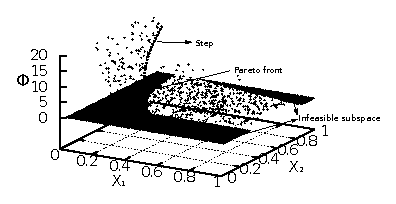
\includegraphics{fit_old.eps}}
\end{minipage}
\caption{Fitness plot for 1000 randomly chosen individuals over the 2d design space of a two-objective constrained optimization problem (fig.\ref{case}) using the traditional penalization method (eq.\ref{penal}) to handle the constraints and SPEAII as fitness assignment algorithm. Constrained region is denoted with grey. "Step" represents the non-uniformity of the near border region, sharp increase in $\Phi$ along the boarder. The Pareto front for the optimization case is located on the left hand side of the border between feasible and infeasible region as shown on the figure.}
\label{fit1}
\end{figure}

To overcome this it is proposed to move the application of penalty from the objective vector directly to the fitness value. So fitness evaluation takes place as if the problem was without constraints ($\Phi(\vec{x})=\Phi(\vec{F}(\vec{x}))$) and the penalization equation (eq.\ref{penal}) is transformed into; 


\begin{eqnarray}
	\Phi(\vec{x})=\Phi(\vec{x})+ \prod _{k=1}^K{\left\{ 				\begin{array}{ll}
    exp(a_k\frac{c_k(x)-d_k}{d_k^* -d_k}) & ~~,c_k(x)>d_k\\
    1 & ~~,c_k(x)\leq d_k\end{array} \right. }
    \label{penal2}
\end{eqnarray}  
where, in comparison with eq.(\ref{penal}), the control vector $\vec{A}$ vanishes and $\vec{a}$ remains to control the penalization intensity for each individual constraint.

\begin{figure}[h!]
\begin{minipage}[b]{1.0\linewidth}
 \centering
 \resizebox*{15cm}{!}{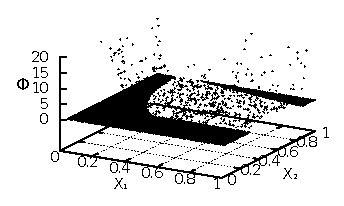
\includegraphics{fit_new.eps}}
\end{minipage}
\caption{Fitness plot for the same 1000 individuals of fig.\ref{fit1} of the same optimization problem but this time using the adapted penalization formulation (eq.\ref{penal2}). Fitness value increases uniformly as the individuals move further into the infeasible subspace (no "step").}
\label{fit2}
\end{figure}
 
\subsection{Generalized Evolutionary Algorithm}

The generalized EA (GEA) used as the algorithmic basis of this thesis is described next.
Each generation $g$ of a GEA is associated with three dynamically updated populations. The offspring $P_{\lambda}^g$ population containing $\lambda$ offsprings, the parent $P_{\mu}^g$ population containing $\mu$ parents and the elite $P_{e}^g$ population containing $e$ elites. $P_{e}^g$ contains the current best Pareto front approximation. Depending on variable coding (binary, binary grey or real), appropriate evolution operators should be applied. 

The GEA as proposed by (cite Giotis 2003, na valo to elliniko didaktoriko?):
\begin{itemize}
\item[]{\bf step 1:}  (Initialization), $g=0$, $P_{\mu}^g=0$ and $P_{\mu}^g=0$. All members of $P_{\lambda}^1$ are initialized using a, within the design bounds,  pseudo-random number generator. Injection of user defined individuals in the initial population is also possible. 
\item[]{\bf step 2:}  (Evaluation), for every individual in $P_{\lambda}^g$, the vector $\vec{F}(\vec{x}) \in \Re^{M} $ is evaluated. In engineering problems evaluation is the most computationally demanding step.
\item[]{\bf step 3:}  (Fitness assignment), for each and every individual $\vec{x} \in P^g$ where, $P^g = P_{\lambda}^g \cup P_{\mu}^g \cup P_{e}^g$ a scalar fitness $\Phi(\vec{x})$ value is assigned.
\item[]{\bf step 4:}  (Elite selection), from population $P^*$ where $P^*=P_{\lambda}^g \cup P_{e}^{g-1}$ the $e^*$ not dominated individuals are selected to enter $P_e^g$. If $e^* > e$ a dilution operator is applied to remove $e^* - e$ neighbouring individuals.     
\item[]{\bf step 5:}  (Elitism), a number of user-specified elite individuals replace the worst members of $P_{\lambda}^g$.  
\item[]{\bf step 6:}  (Parent selection), Parent population is selected from $P_{\mu}^{g-1}$ , $P_{\lambda}^g$ taking into account the maximum generation limit (allowed age, in generations) $k$ for each parent. $P_{\mu}^{g}=S(P_{\mu}^{g-1},P_{\lambda}^g,k)$ 
\item[]{\bf step 7:}  (Recombination and mutation), $P_{\lambda}^{g+1}$ is generated from 
$P_{\mu}^{g}$  by applying the recombination and mutation operators. Recombination $\mathcal{R}(P_{\mu}^{g})$ is the process of combining the genotype of $n$ parents to create one offspring. The second step for the creation of $P_{\lambda}^{g+1}$ is the application of mutation operator. Mutation is the process that randomly changes one part of an individuals genotype $P_{\lambda}^{g+1} = \mathcal{M}(\mathcal{R}(P_{\mu}^{g}))$.
\item[]{\bf step 8:}  (Finalise check) Unless a finalisation criteria is met, return to $step 2$.
\end{itemize}
Hereafter an evolutionary algorithm with $\mu$ parents and $\lambda$ offspring will be referred to as EA($\mu,\lambda$)   

\begin{table}[htdp]
\centering
\begin{tabular}{lr} 
\hline
\hline
number of objectives & M\\
number of design variables & N\\
number of constraints   & K\\
\hline
candidate solution   & x\\
objectives vector  & F\\
constraints vector  & C\\
fitness values & $\Phi$ \\
\hline
\hline
\end{tabular}
\caption[GEA nomenclature]{GEA nomenclature}
\label{GEA nomenclature} 
\end{table}


\subsection{Evolution operators}
Evolution operators are the operators that evolve each generation to the next. This operators are namely; the parent selection operator, the recombination operator, the mutation operator and the elitism operator. This operators will be presented here.
   
\paragraph{Parent selection}
Parent selection purpose is to assign to a selected group of individuals the ability to undergo recombination. The most common parent selection techniques are presented here; 
\begin{itemize}
\item[]{\bf a) Proportional selection.} Selection is based on assigning to each member of the population a probability to be a parent proportional to its fitness value $\Phi$. This is implemented via a roulette wheel algorithm where each and every member of the population receives a portion of the roulette wheel analogous to its $\Phi$, the wheel gets span $\lambda$ times and $\lambda$ parents are selected. 
\item[]{\bf b) Linear ranking.} In Linear ranking, the population is sorted according to $\Phi$ and placed in a sorted list. The probability to be a parent of each individual depends only on its position in the aforementioned list and not on the actual $\Phi$ value.
\item[]{\bf c) Probabilistic tournament selection.}
In probabilistic tournament selection \cite{goldberg1991} a number of randomly chosen individuals is selected from the population and with a user defined ,typically big, probability the best individual from this group is selected as parent. This process is repeated $\lambda$ times to create the required $\lambda$ parents. Parameters for tournament selection is the tournament size, how many individuals take place at each tournament and probability to select the best one. Typical values are $2-3$ individuals per tournament and $80\%-95\%$ probability to select the best.
\end{itemize}

\paragraph{Recombination}
Since the original formulation of GAs \cite{holland_1975} there has been numerous discussions about the merits of recombination as an evolution operator in EAs. In general the purpose of recombination in an EA is to increase the probability of offspring which are fitter than their parents \footnote{Simply put, recombination is the evolution operator that takes advantage of Schema theorem based building block hypothesis in order to increase the probability of offspring which are fitter than their parents.}. Recombination algorithms are separated in to two big groups respecting the coding of the design variables\footnote{Design variables in EAs can be represented either as strings of binary digits or a vector of real numbers.}, the binary and real coding recombination algorithms. 

\subparagraph{Binary coding recombination} is based on exchanging pieces of the binary string that describes the design vector between the parents in order to create the offspring. Depending of the way this exchange takes place the following types of binary coding recombination exists;
\begin{itemize}
\item[]{\bf a) One point recombination.} 
In the general form of one point binary recombination for $\rho$ parents per offspring, the length of the binary string is divided into $\rho-1$ pieces corresponding to the possible pairings of each of the $\rho$ parents with the best of them with respect to fitness. For each of the aforementioned pairings a random integer $\mathcal{X}$ denotes the crossover point\footnote{Analogous to biological crossover, crossing over point of chromosomes.}. The offspring is produced by receiving the left part of the string piece from one parent of the pairing and the right piece from the other, this procedure repeated for all parings. A 2 parents example is presented below.
\begin{figure}[h!]
\begin{minipage}[b]{1.0\linewidth}
 \centering
 \resizebox*{10cm}{!}{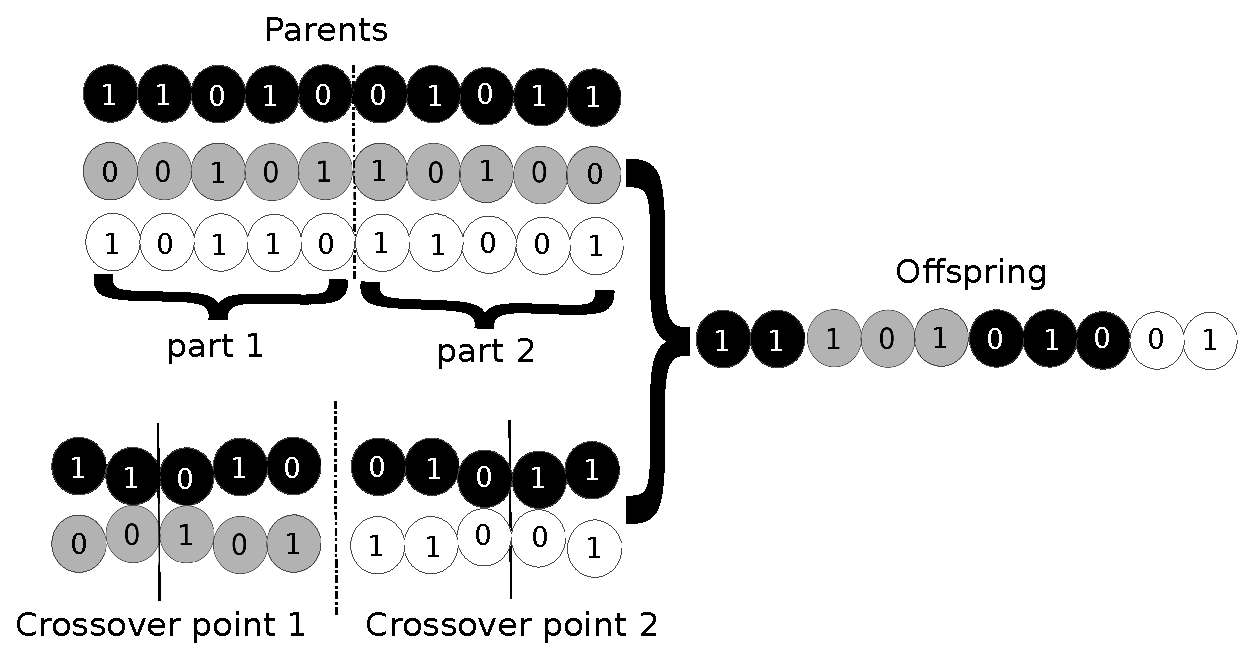
\includegraphics{onepointbinary.eps}}
\end{minipage}
\label{onepX}
\end{figure}
\pagebreak    
\item[]{\bf b) Two point recombination}, shares the same algorithm as one point recombination only this time two crossover points are in use ($\mathcal{X}_1~\&~\mathcal{X}_2$).

\begin{figure}[h!]
\begin{minipage}[b]{1.0\linewidth}
 \centering
 \resizebox*{10cm}{!}{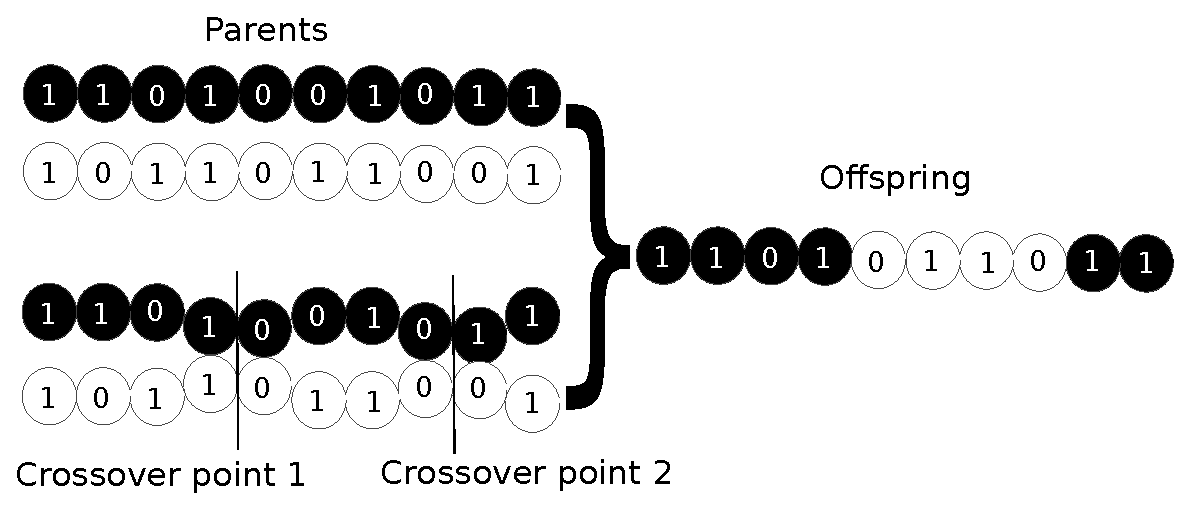
\includegraphics{twopointbinary.eps}}
\end{minipage}
\label{onepX}
\end{figure}

\item[]{\bf c) One or more point recombination per design variable}. Here the aforementioned one and two point recombination techniques are applied to the portions of the binary string that define each design variable separately.  
\end{itemize}
  

\subparagraph{Real coding recombination} as opposed to binary coding recombination is applied not on the binary string that represents the vector of the design variables $\vec{x}$ but directly on the real design variables. The available real coding recombination types are listed below;  

\begin{itemize}
\item[]{\bf a) One point or two recombination.} The techniques of one and two point recombination as proposed for binary coding are transferred to real coding by exchanging  pieces of the design vector $\vec{x}$ instead of pieces of binary strings plus a mixing faction applied on the variables on the vicinity of the crossover point.

\begin{figure}[h!]
\begin{minipage}[b]{1.0\linewidth}
 \centering
 \resizebox*{10cm}{!}{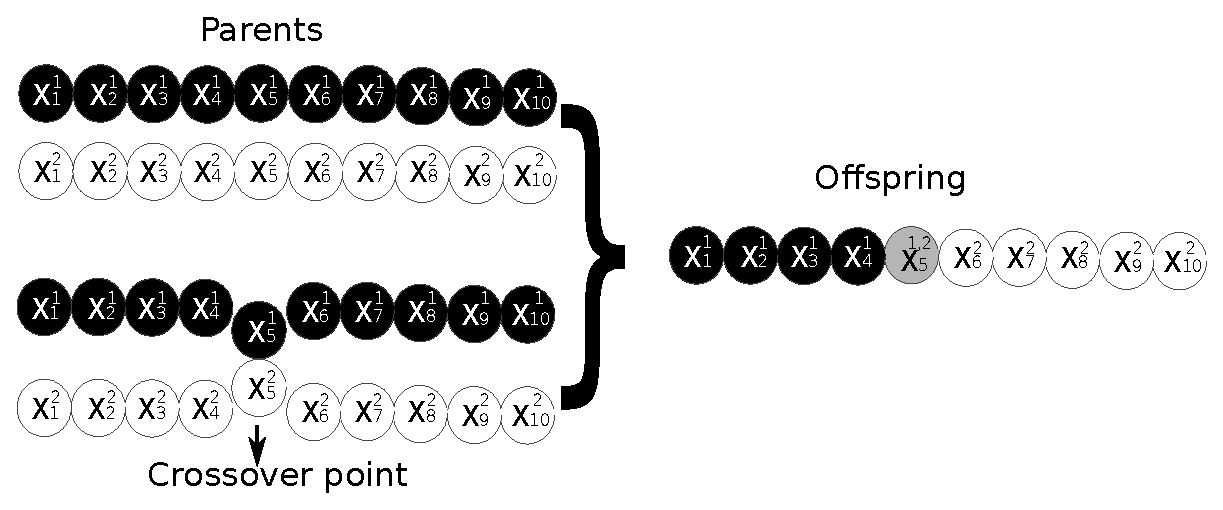
\includegraphics{pointreal.eps}}
\end{minipage}
\label{onepX}
\end{figure}
where, $x_5^{1,2}=x_5^{1}+r(x_5^{2}-x_5^{1}),~ r$ a random number uniformly distributed in $[0,1]$ ($r \in U(0,1)$).    
    
\item[]{\bf b) Discrete recombination.} In discrete recombination each component of $\vec{x}$ for the offspring has $50\%$ probability to be copied either form the best parent $\vec{x}^1$ or from a randomly chosen among the $\rho-1$ remaining ones $\vec{x}^{random}$. 

\begin{figure}[h!]
\begin{minipage}[b]{1.0\linewidth}
 \centering
 \resizebox*{10cm}{!}{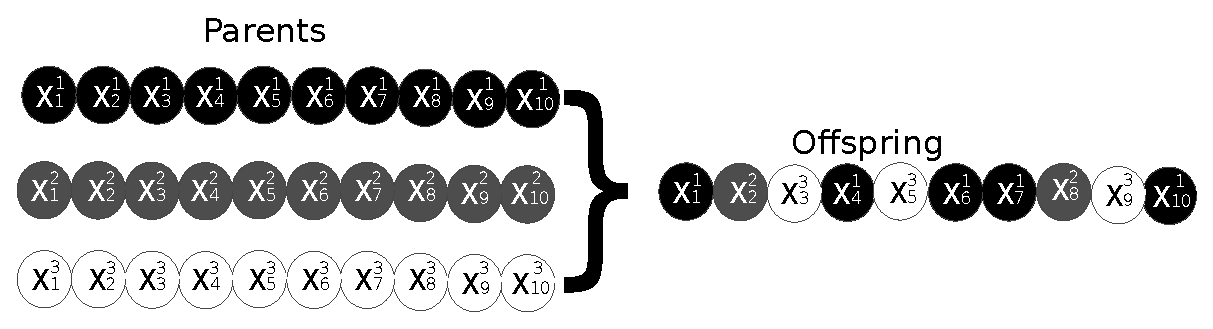
\includegraphics{discrete.eps}}
\end{minipage}
\label{onepX}
\end{figure}
where, $\vec{x^1}$ is the best parent.    
    
\item[]{\bf c) Generalized intermediate recombination}.  In Generalized intermediate recombination each component of $\vec{x}$ is a linear combination of $\vec{x}^1$ and a randomly chosen among the $\rho-1$ remaining ones $\vec{x}^{random}$.
\begin{eqnarray}
\nonumber
\vec{x}=\vec{x}^1+r(\vec{x}^{random}-\vec{x}^1),~ r\in U[0,1]
\end{eqnarray}  
 
\item[]{\bf d) Simulated binary crossover}. Simulated binary crossover (SBX) was design with respect to one-point binary recombination properties of; a) average property \footnote{The average of the decoded parameter values is the same
before and after the crossover operation.} and b) spread factor property \footnote{The probability of occurrence of spread factor $\beta \approx 1$ is more likely than any other $\beta$ value. Spread factor $\beta$ has values close to one when the offspring are similar to the parents.}\cite{SBX1}. The offspring $\vec{x}$ is generated as follows;
\begin{eqnarray}
	\vec{x}={\left\{ 
	\begin{array}{ll}
    \vec{\overline{x}} - \frac{\beta}{2} \times (\vec{x}^{random}-\vec{x}^1)~~,\mbox{if $(r < 0.5)$}\\
	\vec{\overline{x}} + \frac{\beta}{2} \times (\vec{x}^{random}-\vec{x}^1)~~,\mbox{if $(r \geq 0.5)$}
    \end{array} \right. }
    \label{sbxx}
\end{eqnarray}  
where $r\in U[0,1]$, $\vec{\overline{x}}=mean(\vec{x}^{random},\vec{x}^1)$  and 
\begin{eqnarray}
	\beta={\left\{ 
	\begin{array}{ll}
    (2r)^{n}~~~~~~,\mbox{if $(r \leq 0.5)$}\\
	\left(\frac{1}{2r}\right)^{n+2}~~,\mbox{if $(r > 0.5)$}
    \end{array} \right. }
    \label{betasbx}
\end{eqnarray}

Because $r\in U[0,1]$ the probability distribution of $\beta$ can be plotted for various $n$ based on eq.\ref{betasbx} (fig.\ref{sbx}-left). Based on the $\beta$ probability distribution and eq.\ref{sbxx} the probability distribution of offspring as a faction of $n$ and the parents can be plotted (fig.\ref{sbx}-right for a 1d problem and fig.\ref{sbx2} for a 2d problem). In general bigger $n$ values cause higher probability of $\beta \approx 1$ which leads to hight probability of offspring being similar to their parents (spread factor property). Together with the symmetrical offspring probability distribution with respect to $\vec{\overline{x}}$ (average property) the above setup can efficiently simulate one point binary crossover ergo "SBX".    

\begin{figure}[h!]
\begin{minipage}[b]{0.5\linewidth}
 \centering
 \resizebox*{7cm}{!}{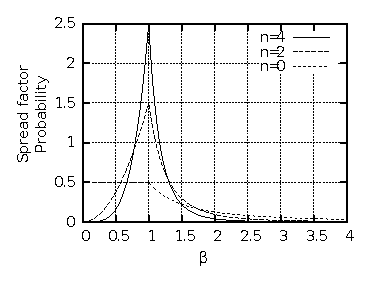
\includegraphics{SBX.eps}}
\end{minipage}
\begin{minipage}[b]{0.5\linewidth}
 \centering
 \resizebox*{7cm}{!}{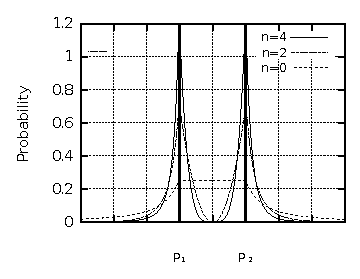
\includegraphics{SBXparents.eps}}
\end{minipage}
\caption{Left: the probability distribution of $\beta$ is plotted for various $n$. Increasing $n$ leads to grater probability of $\beta \approx 1$, $n$ values ranging from $2$ to $5$ are proposed in literature. Right: the offspring probability distribution of a 1d problem is plotted as a faction of the parents $x^1$ and $x^{rand}$ and the value of $n$ }
\label{sbx}
\end{figure}

\begin{figure}[h!]
\begin{minipage}[b]{0.5\linewidth}
 \centering
 \resizebox*{8cm}{!}{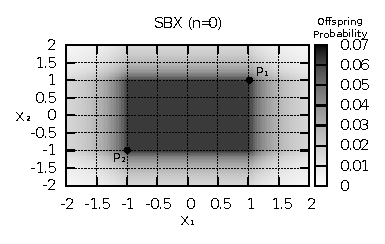
\includegraphics{SBX3dparents0.eps}}
\end{minipage}
\begin{minipage}[b]{0.5\linewidth}
 \centering
 \resizebox*{8cm}{!}{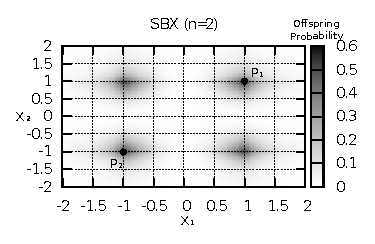
\includegraphics{SBX3dparents2.eps}}
\end{minipage}
\caption{The offspring probability distribution of a 2d, 2 parents ($(1,1),(-1,-1)$) problem is plotted for $n=0$ left and $n=2$ right.}
\label{sbx2}
\end{figure}
\end{itemize}
  
\paragraph{Mutation}
The purpose of mutation in an EA scheme is to introduce and preserve diversity in the population. Thus mutation prevents the population of chromosomes from becoming too similar to each other, thus slowing or even stopping/stagnating the evolution. Mutation is applied on each offspring resulted from recombination subject to a small mutation probability $P_m$. Mutation, as recombination, is also categorized in two groups according with the design variable coding.     

\subparagraph{Binary coding mutation.} In binary coding mutation $P_m$ is applied on each and every bit of the binary string that represents $\vec{x}$ of the individual. For each bit of the binary string there is a probability $P_m$ to switch state from 0 to 1, or vice versa.      

\begin{figure}[h!]
\begin{minipage}[b]{1\linewidth}
 \centering
 \resizebox*{10cm}{!}{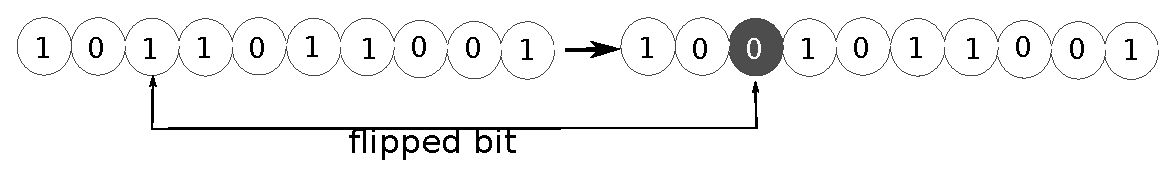
\includegraphics{mut.eps}}
\end{minipage}
\label{binarymut}
\end{figure}

\subparagraph{Real coding mutation.} In real coding mutation $P_m$ is applied on each member of $\vec{x}$. 

\begin{eqnarray}
	\vec{x}_m={\left\{ 
	\begin{array}{ll}
    \vec{x}~~~~~~~~~~,\mbox{if $(P_m > r)$}\\
	N(\vec{x},\vec{\sigma})~,\mbox{if $(P_m \leq r)$}
    \end{array} \right. }
    \label{}
\end{eqnarray}
where $r\in U[0,1]$, $N(\mu,\sigma)$ a normal distribution with mean value = $\mu$ and standard deviation = $\sigma$ and
\begin{eqnarray}
	\vec{\sigma}=\frac{min(\mid \vec{x}-\vec{UB}\mid,\mid \vec{x}- \vec{LB}\mid)}{3} * (1-\frac{g}{g_{max}})^p
	\label{sigmamut} 
\end{eqnarray}
where $\vec{UB}$ and $\vec{LB}$ the vectors of upper and lower bounds for the design variables respectively. $g$ the current generation and $g_{max}$ the maximum allowed generations.$p \simeq 0.2$.

The first part of the eq.\ref{sigmamut} ensures that the mutated individual will respect the design variable bounds and the second part reduces exponentially eith $p$ the magnitude of $\vec{\sigma}$ as the generations advance.

\begin{figure}[h!]
\begin{minipage}[b]{0.5\linewidth}
 \centering
 \resizebox*{7cm}{!}{\includegraphics{Mut_1d.eps}}
\end{minipage}
\begin{minipage}[b]{0.5\linewidth}
 \centering
 \resizebox*{8cm}{!}{\includegraphics{Mut_2d.eps}}
\end{minipage}
\label{realmut}
\caption{Examples of mutant probability distributions for one design variable left $x=0.4$ and two design variable right $\vec{x}=(0.4,0.9)$. For both cases $\vec{LB}=0$ and $\vec{UB}=1$.}
\end{figure}

\paragraph{Elitism}
The purpose of elitism in EAs is to guarantee a mononously improoving course of evolution \cite{Back1996}. In the EA used as algorithmic basis for the thesis elitism operator was generalize with the use of a separate population $P_e^g$ that gets updated every generation as described in GEA-step:4. Furthermore a number of user-specified elite individuals replace the worst members of the offspring population $P^g_{\lambda}$ before the parent selection operator takes place.
  

\section{Metamodel assisted Evolutionary Algorithm}

Due to the involvement of costly evaluation tools (such as CFD tools to numerically predict flows in or around complex 3D geometries), solving engineering optimization problems using EAs may become very computationally demanding. The extensive, smart use of low-cost surrogate evaluation models (often referred to as "metamodels") during the optimization decreases substantially the number of calls to the computationally expensive, problem-specific evaluation code (CFD) making EAs a viable tool that can routinely be used to solve large-scale industrial optimization problems, with affordable wall clock time. Literature surveys on the use of metamodels within EAs can be found in papers \cite{LTT_2_020,Jin2002,LTT_2_027} or books \cite{KEANEbook}.


Polynomial regression, artificial neural networks, Gaussian processes etc. have all been used as metamodels.  Schemes based on different interactions between the metamodel and the problem-specific evaluation tool have been published. Hereafter, all of them will be referred to as MAEAs. This thesis uses the MAEA presented in \cite{LTT_2_018} for SOO and \cite{LTT_2_029} for MOO. 

For all but the first few generations, the metamodels are used to pre-evaluate the current population. Based on the outcome of approximate pre-evaluations, a few most promising individuals are identified and these solely undergo evaluation on the problem-specific evaluation tool to compute their "exact" objective function value(s), before proceeding to the next generation. The $(\mu,\lambda)$ MAEA used herein is sketched in fig.~\ref{MAEA}.


\begin{figure}[h!]
\centering
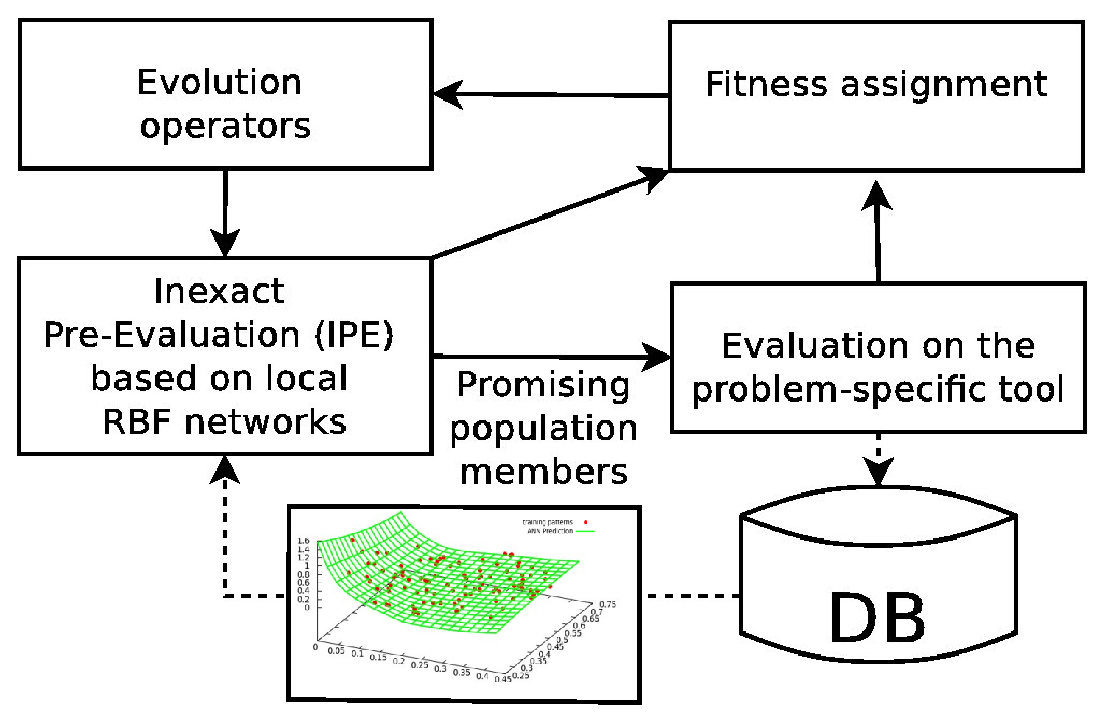
\includegraphics[width=90mm]{MAEA.eps} 
\caption{Schematic representation of the MAEA (namely the variant using on-line trained metamodels) this paper relies on. The loop corresponds to a single EA generation. The so-called inexact pre-evaluation (IPE) phase, within the EA--based search, is used, as described in \cite{LTT_2_020,LTT_2_029}. }
\label{MAEA}
\end{figure}


\paragraph{Radial Basis Function networks enhanced by importance factors}
Herein Radial Basis Function networks (RBFn) are used as metamodels. RBFn are multilayer artificial neural networks (ANN) with three layers, (input,hidden and output) as shown in fig.\ref{rbf1} \cite{Haykin}. Signals propagate through the network in the forward direction, from the input to the output layer, by performing a nonlinear mapping (eq.\ref{RBFa}) followed by a linear one. The latter is related to the weight coefficients $w_l$ that must be computed during the training on a number of available patterns. An RBF network to be used within a MAEA should have $N$ input units, i.e. as many as the  design variables. The hidden layer includes $L$ nodes, associated with the so–called RBF centers $c^l$. At each hidden neuron a nonlinear mapping of the input signals to a single value is carried out using the radial-basis activation function $G:\Re^N \rightarrow \Re$, acting on the distance of input $x$ (eq.\ref{RBFa}) from the corresponding center $c^l \in \Re^N$.  In the current thesis the Gaussian activation is in use. 

\begin{eqnarray}
	G(u,r)=exp(\frac{-u^2}{r^2})
	\label{RBFa}
\end{eqnarray}  
where $u=\Vert x-c^l \Vert_2$ the distance from the corresponding $l^{th}$ RBF center.

\begin{figure}[h!]
\centering
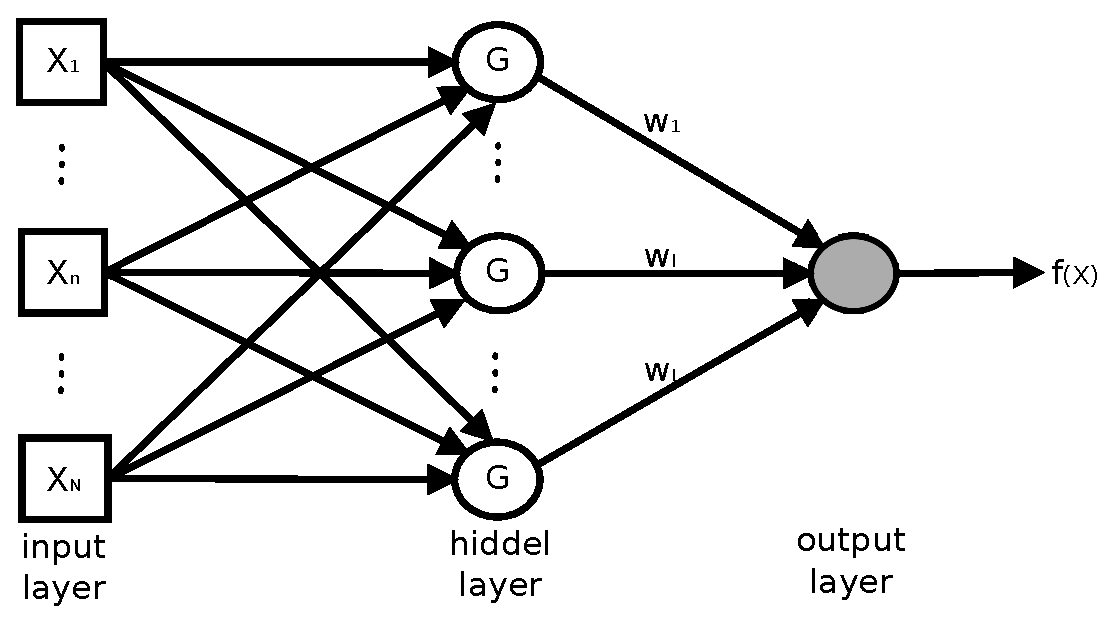
\includegraphics[width=90mm]{RBF.eps} 
\caption{Radial basis function network.}
\label{rbf1}
\end{figure}
The values that the radii or widths r take on may considerably affect the prediction abilities of the network; these are computed using heuristics,\cite{Haykin}. The output layer includes as many nodes as the responses of the network. The single response we are dealing with is expressed by the sum of the weighted output signals from the hidden neurons, as follows             
\begin{eqnarray}
	f(x)=\sum _1^N w_i*G(u(x_i),r)
\end{eqnarray}  


\section{Hierarchical Evolutionary Algorithm}
Typically in engineering design a number of tools with different fidelity and cost (computational and/or economical) are available and used in different steps of the design procedure (fig.\ref{HMAEA} right). Relatively fast low fatality tools are used in the initial stages of the design in order to efficiently scan the design space and high fatality slow (and/or expensive with respect to licensed software or laboratory time) tools are used for the latter steps of design for fine-tuning. In case of turbo-machinery design, for example, a potential code can be used as a low fidelity tool followed by dense or coarse grid Euler codes, Navier-Stokes codes for a single flow passage or the full machine and finally actual laboratory test and adaptation cycles.    


\begin{figure}[h!]
\begin{minipage}[b]{1.0\linewidth}
 \centering
 \resizebox*{13cm}{!}{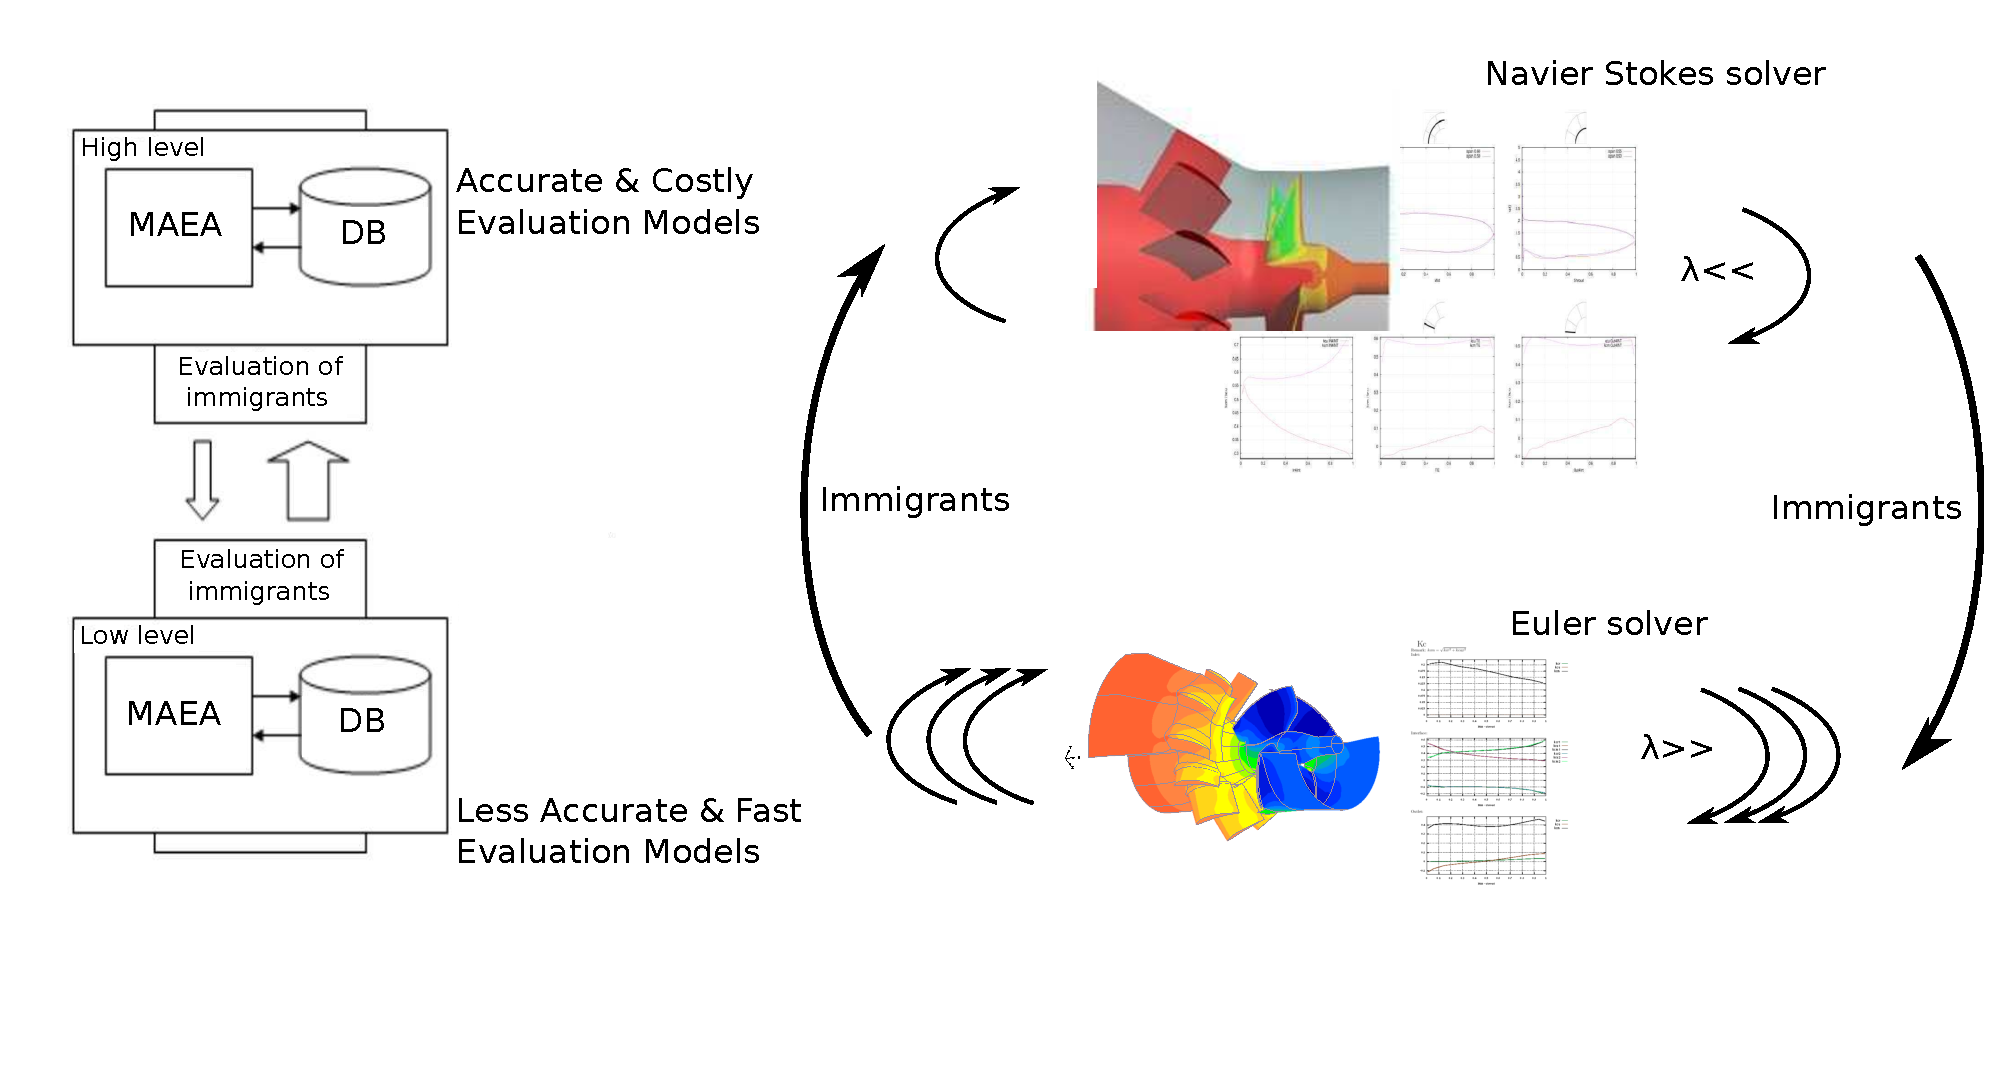
\includegraphics{handmade.eps}}
\end{minipage}
\caption{Left, schematic representation of a two level HMAEA (Hierarchical metamodel assisted evolutionary algorithm). High level is associated with the expensive and accurate tool and lower level with the cheap but not so accurate tool. Communication between the two level is possible in both directions including re-evaluation with the receiving levels evaluation tool. Right, example of two level design procedure as used in industry. A relatively big number of designs is evaluated with the Euler solver once a good design is located it is evaluated with the Navier-Stokes solver. Possible faults are identified, targets for the lower level are updated, that would result in the  elimination of the aforementioned faults, bye experienced designers.}
\label{HMAEA}
\end{figure} 
 
In order to exploit the availability of this tools Hierarchical evolutionary algorithms (HEA) where devised (cite Kampolis + papers). HEA are enhanced EA variants which utilise a number of evolution Levels, each level assigned a different evaluation tool (fig.\ref{HMAEA} left). This multilevel search mechanism splits the computational burden among the levels. On the lower levels, a low cost exploration of the search space is carried out through global search methods, less demanding or less accurate evaluation tools or by even using reduced design variable sets, etc. On the other hand the higher levels undertake the fine-tuning part of the design procedure through denser parameterization, more accurate evaluation tools and/or stochastic or deterministic search methods. These levels mainly serve to refine immigrants from the lower levels. Intercommunication and two-way migrations of individuals between adjacent levels are necessary. The number of levels, the frequency of migration and the number of immigrants are user-defined parameters.

% ---------------------------------------------------------------------------
% ----------------------- end of thesis sub-document ------------------------
% ---------------------------------------------------------------------------